\chapter{\hlc[red]{Discussion \& Conclusion}} \label{ch:conclusion}

\section{\hlc[red]{Summary and Contributions}}

\subsection{\hlc[red]{Theory \& Critical Analysis}}

\subsection{\hlc[red]{The EVDT Framework}}

\subsection{\hlc[red]{Rio de Janeiro Development \& Mangroves}}

\subsection{\hlc[red]{Vida Decision Support System for COVID-19 Response}}

\section{\hlc[red]{Opportunities for Future Inquiry}}

Research Question 3: ``What steps are necessary to establish \ac{evdt} as a continually development framework, a community of practice, and a growing code repository?"

Research Deliverable 3a: ``An assessment of lessons learned from these \ac{dss} development processes"

Research Deliverable 3b: ``An outline of potential future \ac{evdt} refinement and extension, such as using \ac{evdt} to inform the development of future \ac{eo} systems that are better designed for particular application contexts"

Chapter \ref{ch:conclusion} will review these lessons, including discussing how the case studies would have been performed differently in retrospect.

The second portion of the chapter, Section \ref{sec:critiques}, turns towards to critiques of the literature and the concept of this thesis. It is an attempt to recognize and preemptively address potential pitfalls of the approach taken in this thesis. These are primarily fundamental or ethical concerns, as opposed to mere questions of implementation, the latter of which are largely held for Chapter \ref{ch:conclusion}.

\subsection{\hlc[red]{In Rio de Janeiro \& Mangroves Globally}}

\subsection{\hlc[red]{Lessons from COVID-19}}

\subsection{\hlc[red]{The Future of EVDT}} \label{sec:future}


[** discuss evdt with regard to EO value chain]

\begin{figure}[h]
\centering
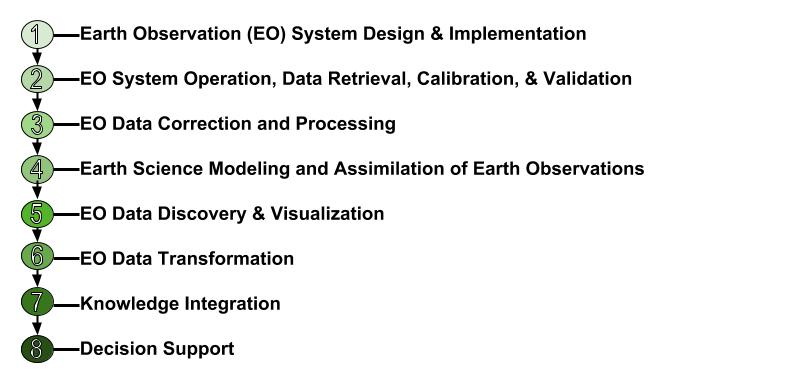
\includegraphics[width=0.9\textwidth]{Figures/chap6/EOChain.jpg}
\caption[Generic Earth Observation Data Value Chain]{Generic Earth Observation Data Value Chain}
\label{fig:eochain}
\end{figure}

the potential of EVDT beyond this thesis 

EVDT is broadly applicable, not just for small geographic projects. Flexible and adaptable.
 (space sustainability)




\section{\hlc[red]{Advancing Stakeholder-Informed Sustainable Development Decision-making}}


